Predstavljanje argumenata u računalima moguće kroz standardne 
serijalizacijske formate, kao što su
XML \engl{Extensible Markup Language} ili JSON \engl{JavaScript Object Notation}. 
No, radi se generičkim formatima, koji ne poznaju specifičnosti 
strukture argumenata. Nezavisno razvijeni alati 
za analizu argumentacije kao Araucaria \citep{reed2004araucaria},
Rationale \citep{van2007rationale}
ili Carnedeas \citep{gordon2006carneades}
su razvili vlastiti serijalizacijski format pohrane
argumenata. Kako je potreba za integracijom između tih alata rasla, tako
je i rasla potreba za ujedinjenim formatom za pohranjivanje argumenta. 

\section{Argument Interchange Format}

Standardizacija definiranja računalnog jezika bila je nužna zbog tri glavna razloga:
\begin{enumerate}
    \item razmjena dokumenata kroz različite programske agente (primjerice 
korištenje dokumenata kreiranih u Araucarii u Rationaleu i obratno), 
    \item kompatiblinost argumentacijskih teorija u različitim programskim agentima
(primjerice, Araucaria koristi Toulminovu teoriju, dok Rationale samo poznaje 
Waltonove argumentacijske teorije \citep{walton2012argument}, te 
    \item potrebe da se automatski procesiraju logičke izjave
\end{enumerate}

Prije AIF-a bilo je nekoliko pokušaja stvaranja zajedničkog jezika, ponajprije
Araucarin AML \engl{Argument Markup Language}. AML, baziran na XML-u
\engl{Extensible Markup Language} osmišljen je za označavanje i analizu
argumentacije u prirodnom jeziku. Sintaksa AML jezika specificirana je pomoću
DTD \engl{Document Type Definition} strukturalnih ograničenja.  
2005.\ nastao je prvi prijedlog za \textbf{AIF} \engl{Argument
Interchange Format} jezik \citep{chesnevar2006towards}. 
Baziran na dobro poznatom RDF jeziku, ideja AIF-a
je bila ponuditi dovoljnu ekspresivnost kojom bi se obuhvatile sve
općeprihvaćene teorije argumentacije i efikasno pohranili 
argumenti u računalima. 
AIF je 2008.\ dobio proširenje za dijalog \citep{reed2008aif+}.
Začetak AIF-a se smatra prvim korakom
prema ostvarivanju argument web-a. 


\section{Specifikacija AIF-a}

AIF odlikuju 
\begin{enumerate*}
    \item sintaksa razumljiva programskim agentima,
    \item eksplicitna semantika,
    \item koncepti i proširenja te
    \item objedinjen apstraktni model koncepata i relacija između
koncepata.
\end{enumerate*}

\subsection{Koncepti i relacije}

Objekti argumentacije predstavljaju se kao skup čvorova povezanih usmjerenim grafom. 
Neformalno se takav usmjereni graf u kontekstu argumentacije naziva
argumentativnom mrežom \engl{argument network} \textbf{AN}. Ne 
postoje nikakva ograničenja na oblik grafa koji može poprimiti AN.

\subsection{Čvorovi}

Razlikujemo dvije osnovne vrste \textbf{čvorova}: informacijske čvorove
\engl{information nodes} I-čvorove i shematske \engl{scheme nodes} S-čvorove.
I-čvorovi predstavljaju sadržaj izjava i čvrsto su povezani s temom
argumentativne rasprave, S-čvorovi predstavljaju primjenu obrazaca u
argumentiranju i smatraju se neovisnim o argumentativnoj raspravi. Postoje tri
osnovna tipa obrasca u argumentiranju: posljedica \engl{inference},
preferiranje \engl{preference} i sukob \engl{conflict}. Primjena sheme
radi se kroz S-čvor koji sukladno vrstama obrazaca u argumentiranju može biti
čvor primjene logičke posljedice \engl{inference application node} (\textbf{RA-čvor}), 
čvor primjene preferiranja \engl{preference application node} (\textbf{PA-čvor}) te
čvor primjene sukoba \engl{conflict application node} (\textbf{CA-čvor}).

\subsection{Bridovi}

\textbf{Čvorovi} su povezani usmjerenim bridovima. Kažemo da brid povezuje čvorove $A$ i $B$
tako da ide iz početnog čvora $A$ u odredišni čvor $B$. Razlikujemo shematske i podatkovne
bridove. Početne točke shematskih bridova su S-čvorovi, dok su početne točke 
podatkovnih bridova I-čvorovi. Primjerice, čvorovi $A$ i $B$ su povezani usmjerenim bridom 
$A \rightarrow B$. Ukoliko je čvor $A$ početna točka tipa
S-čvor primjene logičke posljedice RA-čvor onda je čvor $B$ zaključak strukture
čvora $A$. Čvor $B$ može biti S-čvor ili I-čvor. Ukoliko je početni čvor I-čvor onda
odredišni čvor može biti samo S-čvor. 
Ideja iza toga stoji u principu da nije moguće povezati dvije izjave bez da se
specifira relacija (S-čvor) između izjava. 
\cite{chesnevar2006towards} navode sve moguće kombinacije S-čvorova i I-čvorova
sa bridovima uz pripadajuće semantičko značenje. 

\section{Primjeri AIF dokumenta}
\label{sec:primjeri}

AIF dokumente moguće je preslikavati u raznim formatima: 
\textbf{OWL/RDF}, \textbf{AML}(format kompatibilan sa sustavom Araucaria), 
\textbf{RTNL} (format kompatibilan sa sustavom Rationale), 
\textbf{LKIF} (format kompatibilan sa sustavom Carnedeas), \textbf{DOT} \engl{graph 
description language} i \textbf{SVG} \engl{scalable vector graphics} format. 
U nastavku će se prikazati jednostavan AIF dokument istovjetnog sadržaja 
u različitim formatima. AIF dokument sadrži tvrdnje: 
\begin{exe}
    \ex\label{ex5} \emph{Student Ivo je predao seminar}
    \ex\label{ex6} \emph{Student Ivo nije pristupio ispitu iz PZUIS-a} i
    \ex\label{ex7} \emph{Student Ivo bi trebao položiti PZUIS}.
\end{exe}
Tvrdnja (\ref{ex7}) logički slijedi iz tvrdnje (\ref{ex5}), dok tvrdnja (\ref{ex6})
je u kontradikciji sa tvrdnjom (\ref{ex7}). Između tvrdnji (\ref{ex5}) i (\ref{ex6}) 
nema logičke veze. 

\subsection{XML RDF primjer AIF dokumenta}

Primjer isječka AIF dokumenta u XML RDF formatu vidljiv je kodu~\ref{lst:aif_rdf}.
Tip čvora definiran je kroz \textit{rdf:type} (I-čvor ili S-čvor),
\textit{aif:claimText} predstavlja sadržaj I-čvora, dok S-čvor ima ima različita
svojstva (ovisno o tome radi li se o RA, PA ili CA čvoru). 
U ovom primjeru imamo po jedan S-čvor zaključivanja (RA-čvor) 
i S-čvor primjene sukoba (CA-čvor) koji 
spajaju dva čvora: \textit{aif:Premise} čvor i \textit{aif:Conclusion} čvor. 

\lstset{language=XML}
\begin{lstlisting}[caption={Primjer AIF RDF dokumenta},label={lst:aif_rdf},language=XML, captionpos=b]
<?xml version="1.0"?>
    <!-- http://www.arg.dundee.ac.uk/AIFdb/nodes/319262 -->
    <NamedIndividual rdf:about="&http;www.arg.dundee.ac.uk/AIFdb/nodes/319262">
        <rdf:type rdf:resource="&http;www.arg.dundee.ac.uk/aif#I-node"/>
        <aif:claimText>Student Ivo bi trebao položiti PZUIS</aif:claimText>
        <aif:Conclusion rdf:resource="&http;www.arg.dundee.ac.uk/AIFdb/nodes/319264"/>
        <aif:Conclusion rdf:resource="&http;www.arg.dundee.ac.uk/AIFdb/nodes/319266"/>
        <aif:creationDate>2017-12-20 18:17:01</aif:creationDate>
    </NamedIndividual>

    <!-- http://www.arg.dundee.ac.uk/AIFdb/nodes/319263 -->
    <NamedIndividual rdf:about="&http;www.arg.dundee.ac.uk/AIFdb/nodes/319263">
        <rdf:type rdf:resource="&http;www.arg.dundee.ac.uk/aif#I-node"/>
        <aif:claimText>Student Ivo je predao seminar</aif:claimText>
        <aif:Premise rdf:resource="&http;www.arg.dundee.ac.uk/AIFdb/nodes/319264"/>
        <aif:creationDate>2017-12-20 18:17:01</aif:creationDate>
    </NamedIndividual>

    <!-- http://www.arg.dundee.ac.uk/AIFdb/nodes/319264 -->
    <NamedIndividual rdf:about="&http;www.arg.dundee.ac.uk/AIFdb/nodes/319264">
        <rdf:type rdf:resource="&http;www.arg.dundee.ac.uk/aif#RA-node"/>
        <aif:Premise rdf:resource="&http;www.arg.dundee.ac.uk/AIFdb/nodes/319263"/>
        <aif:Conclusion rdf:resource="&http;www.arg.dundee.ac.uk/AIFdb/nodes/319262"/>
        <aif:creationDate>2017-12-20 18:17:02</aif:creationDate>
    </NamedIndividual>

    <!-- http://www.arg.dundee.ac.uk/AIFdb/nodes/319265 -->
    <NamedIndividual rdf:about="&http;www.arg.dundee.ac.uk/AIFdb/nodes/319265">
        <rdf:type rdf:resource="&http;www.arg.dundee.ac.uk/aif#I-node"/>
        <aif:claimText>Student Ivo nije pristupio ispitu iz PZUIS-a.</aif:claimText>
        <aif:Premise rdf:resource="&http;www.arg.dundee.ac.uk/AIFdb/nodes/319266"/>
        <aif:creationDate>2017-12-20 18:17:02</aif:creationDate>
    </NamedIndividual>

    <!-- http://www.arg.dundee.ac.uk/AIFdb/nodes/319266 -->
    <NamedIndividual rdf:about="&http;www.arg.dundee.ac.uk/AIFdb/nodes/319266">
        <rdf:type rdf:resource="&http;www.arg.dundee.ac.uk/aif#CA-node"/>
        <aif:Premise rdf:resource="&http;www.arg.dundee.ac.uk/AIFdb/nodes/319265"/>
        <aif:Conclusion rdf:resource="&http;www.arg.dundee.ac.uk/AIFdb/nodes/319262"/>
        <aif:creationDate>2017-12-20 18:17:02</aif:creationDate>
    </NamedIndividual>
\end{lstlisting}

\subsection{AML primjer AIF dokumenta}

Primjer isječka AIF dokumenta u AML formatu vidljiv je kodu~\ref{lst:aif_aml}.
U AML formatu čvorovi nisu eksplicitno definirani, već
strutkura ima oblik n-arnog stabla. Čvor stabla odgovara I-čvoru, dok je S-čvor
definiran kroz tip veze koja povezuje čvor sa djetetom. U kodu~\ref{lst:aif_aml}
vidimo da je tvrdnja (\ref{ex7}) korijen stabla 
povezan sa CA-čvorom (\emph{CA}) prema djetetu
(\ref{ex5}) i RA-čvor (\emph{REFUTATION}) vezom prema čvoru (\ref{ex6}).

\lstset{language=XML}
\begin{lstlisting}[caption={Primjer AIF AML dokumenta},label={lst:aif_aml},language=XML, captionpos=b]
<?xml version="1.0" encoding="UTF-8"?>
<!DOCTYPE ARG SYSTEM "argument.dtd">
<ARG>
  <?Araucaria UTF-8?>
  <AU>
    <PROP identifier="A" missing="yes">
      <PROPTEXT offset="-1">Student Ivo bi trebao položiti PZUIS</PROPTEXT>
    </PROP>
    <REFUTATION>
      <AU>
        <PROP identifier="B" missing="no">
          <PROPTEXT offset="274">Student Ivo nije pristupio ispitu iz PZUIS-a.</PROPTEXT>
        </PROP>
      </AU>
    </REFUTATION>
    <CA>
      <AU>
        <PROP identifier="C" missing="no">
          <PROPTEXT offset="99">Student Ivo je predao seminar</PROPTEXT>
        </PROP>
      </AU>
    </CA>
  </AU>
</ARG>
\end{lstlisting}

\subsection{RTNL primjer AIF dokumenta}

Rationale sustav koristi format sličan Python kodu. 
Primjer AIF dokumenta u RTNL formatu vidljiv je u kodu~\ref{lst:aif_rtnl}.
Slično kao u AML-u, u RTNL-u se gradi n-arno stablo gdje vrsta
veze prema djeci definira tip S-čvora. 


\begin{lstlisting}[caption={Primjer AIF RTNL dokumenta},label={lst:aif_rtnl},language=Python, captionpos=b]
Node = None

def CreateChild(parent, type):
   global Node
   Node = app.CreateChild(parent, type)
   return Node

def SetText(text):
   app.SetText(Node, text)

map0_0 = Create("Claim")
SetText("Student Ivo bi trebao položiti PZUIS")
map1_1 = CreateChild(map0_0, "CompoundReason")
map1_2 = CreateChild(map1_1, "Claim")
SetText("Student Ivo je predao seminar")
map1_3 = CreateChild(map1_1, "Inference")
map1_4 = CreateChild(map0_0, "CompoundObjection")
map1_5 = CreateChild(map1_4, "Claim")
SetText("Student Ivo nije pristupio ispitu iz PZUIS-a.")
map1_6 = CreateChild(map1_4, "Inference")
\end{lstlisting}

\subsection{LKIF primjer AIF dokumenta}

Primjer AIF dokumenta u LKIF formatu vidljiv je u kodu~\ref{lst:aif_lkif}.
Carnedeasov format je nešto sličniji AML-ovom i RDF XML AIF-ovom. 
Prvo se nabrajaju sve tvrdnje u \emph{statements} oznaci (tagu), koje odgovaraju I-čvorovima, 
dok se kroz \emph{arguments} definiraju S-čvorovi s pripadajućim tipom (\emph{scheme}).

\lstset{language=XML}
\begin{lstlisting}[caption={Primjer AIF LKIF dokumenta},label={lst:aif_lkif},language=XML, captionpos=b]
<?oxygen RNGSchema="../../schemas/LKIF2.rnc" type="compact"?>
<lkif version="2.0.4">
  <argument-graphs>
      <argument-graph id="NewGraph" title="New Graph">
          <statements>
            <statement assumption="true" id="319262" standard="BA" value="unknown">
              <s>Student Ivo bi trebao položiti PZUIS</s>
            </statement>
            <statement assumption="true" id="319263" standard="BA" value="unknown">
              <s>Student Ivo je predao seminar</s>
            </statement>
            <statement assumption="true" id="319265" standard="BA" value="unknown">
              <s>Student Ivo nije pristupio ispitu iz PZUIS-a.</s>
            </statement>
          </statements>
          <arguments>
            <argument direction="pro" id="319264" scheme="Default Inference" weight="0.5">
              <conclusion statement="319262"/>
              <premises>
                <premise polarity="positive" type="ordinary" role="" statement="319263"/>
              </premises>
            </argument>
            <argument direction="con" id="319266" scheme="Default Conflict" weight="0.5">
              <conclusion statement="319262"/>
              <premises>
                <premise polarity="positive" type="ordinary" role="" statement="319265"/>
              </premises>
            </argument>
          </arguments>
      </argument-graph>
  </argument-graphs>
</lkif>
\end{lstlisting}

\subsection{DOT primjer AIF dokumenta}

DOT prikaz tipičan je za prikaz grafova, pa je stoga pogodan za prikaz
argumentacije i mreže argumenata. 
Primjer AIF dokumenta u DOT formatu vidljiv je u kodu~\ref{lst:aif_dot}.
Čvorovi u DOT formatu odgovaraju čvorovima. Oznaka čvora (\emph{label})
označava tip čvora, s time da u DOT formatu nema hijerarhije vrsta čvorova 
(nema apstraktnih S-čvorova, već samo RA, PA ili CA-čvorova). Čvorovi su
povezani jednostavnim usmjerenim vezama (označenim $\rightarrow$).

%\lstset{language=XML}
\begin{lstlisting}[caption={Primjer AIF DOT dokumenta},label={lst:aif_dot},captionpos=b]
digraph nodeset13108 {
 319262 [label="Student Ivo bi trebao\npoložiti PZUIS"];
 319263 [label="Student Ivo je predao seminar"];
 319264 [label="Default Inference"];
 319265 [label="Student Ivo nije pristupio\nispitu iz PZUIS-a."];
 319266 [label="Default Conflict"];
319264 ->; 319262; 319263 ->; 319264; 319266 ->; 319262; 319265 ->; 319266;}
\end{lstlisting}

\subsection{SVG primjer AIF dokumenta}

SVG format definira vektorizirane objekte i većina preglednika slika podržava 
prikaz SVG datoteka. 
Primjer AIF dokumenta u SVG XML formatu vidljiv je u kodu~\ref{lst:aif_svg}.
U slučaju SVG formata najteže je doći do argumentacijske mreže sa gledišta parsiranja dokumenta, 
ponajviše jer je prioritet SVG formata prikaz slike pa su podaci nisu strukturirani tako da se
kroz jednu oznaku (tag) može pronaći I-čvor ili S-čvor. 

\lstset{language=XML}
\begin{lstlisting}[caption={Primjer AIF SVG dokumenta},label={lst:aif_svg},language=XML, captionpos=b, basicstyle=\scriptsize]
<?xml version="1.0" encoding="UTF-8"?>
<svg xmlns="http://www.w3.org/2000/svg" xmlns:xlink="http://www.w3.org/1999/xlink" width="336pt" height="188pt" viewBox="0.00 0.00 336.00 188.00">
  <g id="graph1" class="graph" transform="scale(1 1) rotate(0) translate(4 184)">
    <title>nodeset13108</title>
    <polygon fill="white" stroke="white" points="-4,5 -4,-184 333,-184 333,5 -4,5" />
    <!-- 319262 -->
    <g id="node1" class="node">
      <title>319262</title>
      <polygon fill="#ebf3ff" stroke="#6666cc" points="220,-36 114,-36 114,-1.77636e-14 220,-3.55271e-15 220,-36" />
      <text text-anchor="middle" x="167" y="-23" font-family="FreeSans" font-size="10.00">Student Ivo bi trebao</text>
      <text text-anchor="middle" x="167" y="-9" font-family="FreeSans" font-size="10.00">položiti PZUIS</text>
    </g>
    <!-- 319263 -->
    <g id="node2" class="node">
      <title>319263</title>
      <polygon fill="#ebf3ff" stroke="#6666cc" points="154,-180 8,-180 8,-144 154,-144 154,-180" />
      <text text-anchor="middle" x="81" y="-160" font-family="FreeSans" font-size="10.00">Student Ivo je predao seminar</text>
    </g>
    <!-- 319264 -->
    <g id="node3" class="node">
      <title>319264</title>
      <polygon fill="#e6ffe6" stroke="#66cc66" points="81,-108 0.206152,-90 81,-72 161.794,-90 81,-108" />
      <text text-anchor="middle" x="81" y="-88" font-family="FreeSans" font-size="10.00">Default Inference</text>
    </g>
    <!-- 319263&#45;&gt;319264 -->
    <g id="edge4" class="edge">
      <title>319263-&gt;319264</title>
      <path fill="none" stroke="black" d="M81,-143.831C81,-136.131 81,-126.974 81,-118.417" />
      <polygon fill="black" stroke="black" points="84.5001,-118.413 81,-108.413 77.5001,-118.413 84.5001,-118.413" />
    </g>
    <!-- 319264&#45;&gt;319262 -->
    <g id="edge2" class="edge">
      <title>319264-&gt;319262</title>
      <path fill="none" stroke="black" d="M97.9908,-75.7751C109.26,-66.3402 124.348,-53.709 137.541,-42.6634" />
      <polygon fill="black" stroke="black" points="140.039,-45.1367 145.46,-36.0336 135.545,-39.7694 140.039,-45.1367" />
    </g>
    <!-- 319265 -->
    <g id="node4" class="node">
      <title>319265</title>
      <polygon fill="#ebf3ff" stroke="#6666cc" points="316,-180 192,-180 192,-144 316,-144 316,-180" />
      <text text-anchor="middle" x="254" y="-167" font-family="FreeSans" font-size="10.00">Student Ivo nije pristupio</text>
      <text text-anchor="middle" x="254" y="-153" font-family="FreeSans" font-size="10.00">ispitu iz PZUIS-a.</text>
    </g>
    <!-- 319266 -->
    <g id="node5" class="node">
      <title>319266</title>
      <polygon fill="#ffe6e6" stroke="#cc6666" points="254,-108 179.854,-90 254,-72 328.146,-90 254,-108" />
      <text text-anchor="middle" x="254" y="-88" font-family="FreeSans" font-size="10.00">Default Conflict</text>
    </g>
    <!-- 319265&#45;&gt;319266 -->
    <g id="edge8" class="edge">
      <title>319265-&gt;319266</title>
      <path fill="none" stroke="black" d="M254,-143.831C254,-136.131 254,-126.974 254,-118.417" />
      <polygon fill="black" stroke="black" points="257.5,-118.413 254,-108.413 250.5,-118.413 257.5,-118.413" />
    </g>
    <!-- 319266&#45;&gt;319262 -->
    <g id="edge6" class="edge">
      <title>319266-&gt;319262</title>
      <path fill="none" stroke="black" d="M236.812,-75.7751C225.411,-66.3402 210.148,-53.709 196.802,-42.6634" />
      <polygon fill="black" stroke="black" points="198.726,-39.713 188.791,-36.0336 194.263,-45.1057 198.726,-39.713" />
    </g>
  </g>
</svg>

\end{lstlisting}
\section{AIFdb}
\label{sec:aifdb}


AIFdb\footnote{Dostupan na \url{aifdb.org}} \citep{lawrence2012aifdb} 
je softversko rješenje za pretraživanje, pohranu i vizualizaciju AIF dokumenata te
integraciju s drugim Argument Web alatima. 
Sastoji se od tri dijela:
\begin{enumerate*}
    \item korisničkog sučelja za vizualizaciju AIF dokumenata,
    \item baze podataka koja pohranjuje AIF dokumente i
    \item web servisa koji ima programski pristup bazi podataka.
\end{enumerate*}
Baza podataka pohranjuje dokumente u AIF formatu. 
AIF dokumentima u bazi podataka moguće je pristupati kroz korisničko sučenje 
kroz web preglednik, ili programski, koristeći sučelje web servisa.  
Putem web servisa moguće je pretraživati i pregledavati AIF dokumente. 
U AIFdb moguće je uvesti \engl{import} dokumente u formatima alata 
Carnedeas, Rationale i Araucaria te RDF-XML formatu, te izvoziti \engl{export}
u formatima SVG \engl{support vector graphics}, DOT \engl{graph description language}
RDF te formatima alata Rationale i Carnedeas. 

\begin{figure}[h!]
    \centering
    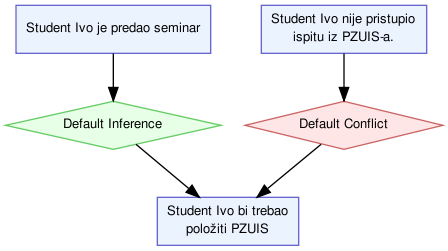
\includegraphics[scale=0.8]{aifdb_ex.png}
\caption{Primjer jednostavnog AIF dokumenta u AIFdb korisničkom sučelju}
\label{fig:aifdb_ex}
\end{figure}

Korisnik može preko web sučelja dodavati AIFdb korpuse \citep{lawrence2014aifdb}, 
koji grupiraju AIF dokumenate. 
Jedan od korpusa dostupan online u AIFdb-u je i Araucaria korpus koji 
u trenutku pisanja sadrži 662 AIF dokumenta. 
Osim pohranjivanja, razmjene i vizualizacije AIF dokumenata, AIFdb je integriran 
s alatima koji evaluiraju arugment u AIF formatu (više u poglavlju~\ref{chap:eval}). 
Jednostavan primjer AIF dokumenta (iz odjeljka~\ref{sec:primjeri})
pohranjen u AIFdb-u je na slici~\ref{fig:aifdb_ex}. Detalje poput sheme 
baze podataka moguće je pronaći u \citep{lawrence2014aifdb} i na web stranicama
centra za tehnologiju argumentacije \engl{Centre for Argument Techology} 
ARG-tech\footnote{Projekti ARG-techa dostupni na \url{http://www.arg-tech.org/index.php/projects/}}.




